% -*- TeX -*- -*- UK -*- -*- Soft -*-

% Front matter
\frontmatter

% r.1 blank page
\blankpage


% r.3 full title page
\maketitle


% v.4 copyright page
\newpage
\begin{fullwidth}
~\vfill
\thispagestyle{empty}
\setlength{\parindent}{0pt}
\setlength{\parskip}{\baselineskip}
Copyright \copyright\ \the\year\ \thanklessauthor, as indicated in the text

%\par\smallcaps{Published by \thanklesspublisher}

\par\smallcaps{https://github.com/NelisW/NeuralNetworks-DeepLearning-Notes}

\par
This work is licensed under a Creative Commons Attribution-
NonCommercial 4.0 Unported License. This means you’re free to
copy, share, and build on this book, but not to sell it. 
You may obtain a copy
of the License at \url{https://creativecommons.org/licenses/by-nc/4.0/}. Unless
required by applicable law or agreed to in writing, software distributed
under the License is distributed on an \smallcaps{``AS IS'' BASIS, WITHOUT
WARRANTIES OR CONDITIONS OF ANY KIND}, either express or implied. See the
License for the specific language governing permissions and limitations
under the License.\index{license}
If you’re interested in commercial use, please contact both the authors.

\par\textit{Current printing, \monthyear}
\end{fullwidth}

% r.5 contents
\tableofcontents

\listoffigures

%\listoftables

% -*- TeX -*- -*- UK -*- -*- Soft -*-
\chapter*{Abbreviations}
%\addcontentsline{toc}{chapter}{ABBREVIATIONS}

% use:
%  \ac{IR}

\begin{acronym}
\acro{2-D}{Two-Dimensional}
\acro{2D}{Two-Dimensional}
\acro{3-D}{Three-Dimensional}
\acro{3D}{Three-Dimensional}
\acro{A2D}{Analogue to Digital}
\acro{AAM}{Air-to-Air Missile}
\acro{AASRAM}{Air-to-Air Short Range Missile}
\acro{AA}{Air-to-Air}
\acro{ACE}{Adaptive Communication Environment}
\acro{AC}{Alternating Current}
\acro{ADC}{Analogue to Digital Converter}
\acro{AD}{Analogue to Digital (conversion)}
\acro{AFB}{Air Force Base}
\acro{AFCRL}{Air Force Cambridge Research Laboratories}
\acro{AFRL}{Air Force Research Laboratories}
\acro{AGC}{Automatic Gain Control}
\acro{AGL}{Above Ground Level}
\acro{AHP}{Analytical Hierarchy Process}
\acro{AI}{Artificial Intelligence}
\acro{AIM}{Air Intercept Missile}
\acro{AIRS}{Atmospheric Infrared Sounder}
\acro{AMBBB}{Ambient Temperature Blackbody}
\acro{AMRAAM}{Advanced Medium Range Air-to-Air Missile}
\acro{AM}{Amplitude Modulation}
\acro{ANSI}{American National Standards Institute}
\acro{API}{Application Programming Interface}
\acro{APU}{Auxiliary Power Unit}
\acro{ASCII}{American Standard Code for Information Interchange}
\acro{ASIC}{Application Specific Integrated Circuit}
\acro{ASL}{Above Sea Level}
\acro{ASRAAM}{Advanced Short Range Air-to-Air Missile}
\acro{ASU}{Air Support Unit}
\acro{ATP}{Acceptance Test Procedure}
\acro{ATR}{Automatic Target Recognition}
\acro{ATS}{Advanced Thermographic Systems}
\acro{AVI}{Audio Video Interleave}
\acro{BAe}{British Aerospace}
\acro{BB}{Black Body}
\acro{BCU}{Battery Coolant Unit}
\acro{BDI}{Buffered Direct Injection}
\acro{BDRF}{Bidirectional Reflection Function}
\acro{BFS}{Bomem File System}
\acro{BGRAMS}{Bomem Grams a software product}
\acro{BGT}{Bodenseewerk Ger\"atetechnik Gmbh}
\acro{BH}{I/O Bulkhead input/output}
\acro{BIT}{Built-in Test}
\acro{BLT}{Bilinear Transformation}
\acro{BNC}{Bayonet Neill-Concelman}
\acro{BPR}{Bad Pixel Replacement}
\acro{BRDF}{Bidirectional Reflectance Distribution Function}
\acro{BSP}{Binary Space Partitions}
\acro{BVR}{Beyond Visual Range}
\acro{C$^4$I$^3$RS}{Command, Control, Communication, Computers, Information, Intelligence, Informatics, Reconnaissance and Surveillance}
\acro{CAD}{Computer Aided Design}
\acro{CAT}{Computed Axial Tomography}
\acro{CCD}{Charge Coupled Device}
\acro{CCIR}{Comite Consultatif International des Radio Communications}
\acro{CCM}{Counter-countermeasure}
\acro{CDSD}{Carbon Dioxide Spectroscopic Database}
\acro{CDS}{Correlated Double Sampling}
\acro{CD}{Compact Disk}
\acro{CEDIP}{Name of the camera manufacturer}
\acro{CFAR}{Constant False Alarm Rate}
\acro{CFI}{Customer Furnished Information}
\acro{CML}{Configurable Math Library}
\acro{CMOS}{Complementary Metal Oxide Semiconductor}
\acro{CmSim2}{Countermeasure Simulator (version 2)}
\acro{CmSim}{Countermeasure Simulator (version 1)}
\acro{CMS}{Classified MicroSeek}
\acro{CMT}{Cadmium Mercury Telluride}
\acro{CnC}{Command and Control}
\acro{CNES}{Centre National d'Etudes Spatiales, France}
\acro{CNR}{Clutter-to-noise ratio}
\acro{CNUC}{Continuous Non-Uniformity Correction}
\acro{CO$_2$}{Carbon Dioxide}
\acro{CODATA}{Committee on Data for Science and Technology}
\acro{COM}{Common Object Model}
\acro{CORBA}{Common Object Request Broker Architecture}
\acro{COTS}{Commercial of the Shelf}
\acro{CPU}{Central Processing Unit}
\acro{CSCI}{Computer Software Configuration Item}
\acro{CSIR}{Council for Scientific and Industrial Research}
\acro{CSV}{Comma Separated Variable}
\acro{CVS}{Concurrent Versions System}
\acro{CTAN}{Comprehensive TeX Archive Network}
\acro{CTIA} {Capacitive Transimpedance Amplifiers}
\acro{CVD}{Chemical vapour deposition}
\acro{DAS}{Denel Aerospace }
\acro{DCS}{Direct Current Subtraction}
\acro{DC}{Direct Current}
\acro{DD}{Denel Dynamics}
\acro{DEMS}{Digital Elevation Maps}
\acro{DEM}{Digital Elevation Map}
\acro{DFPN}{Dark current Fixed Pattern Noise}
\acro{DFT} {Discrete Fourier Transform}
\acro{DIRCM}{Directed Infrared Countermeasure}
\acro{DIRSIG}{Digital Imaging and Remote Sensing Image Generation}
\acro{DITSIM}{Directed Infrared Countermeasure and Imaging Toolkit Simulator}
\acro{DI}{Direct Injection}
\acro{DLE}{Differential Linearity Error }
\acro{DLSWC}{Denel Land Systems Western Cape}
\acro{DLU}{Directed Laser Unit}
\acro{DL}{Digital Level}
\acro{dl}{Digital Level}
\acro{DLea}[DL]{Deep Learning}
\acro{DLL}{Dynamic Load Library}
\acro{DOI}{Digital Object Identifier}
\acro{DPA}{Digital Processing Assembly}
\acro{DPSS}{Defence, Peace Safety and Security, an operating unit of the CSIR}
\acro{DRI}{Detection, Recognition and Identification}
\acro{DSIM}{Directed Infrared Countermeasure Simulator}
\acro{DSP}{Digital Signal Processing}
\acro{DTD}{Document Type Definition}
\acro{DVD}{Digital Video Disk or Digital Versatile Disk}
\acro{ECCM}{Electronic Counter-Countermeasure}
\acro{ECEF}{Earth Centred Earth Fixed}
\acro{EDERI}{Electronic Defence Evaluation and Research Institute}
\acro{EDS}{Electronic Defence Systems}
\acro{EEPROM}{Electronically Erasable Programmable Read-Only Memory}
\acro{EGT}{Exhaust Gas Temperature}
\acro{EICAS}{Engine Indication and Crew Alert System}
\acro{EMC}{Electromagnetic Compatibility}
\acro{EMI}{Electro-magnetic interference}
\acro{EMP}{Electro-magnetic pulse}
\acro{ENU}{East North Up}
\acro{ENVI}{An image processing product}
\acro{EofN}{east of north}
\acro{EOSS}{Electro-Optical Simulation System}
\acro{EO}{Electro Optics}
\acro{EPS}{European Polar System }
\acro{ESD}{East-South-Down (coordinate convention)}
\acro{EULA}{End-User Licence Agreement}
\acro{EUMETSAT}{EUropean organization for the exploitation of METeorological SATellites}
\acro{EWC}{Electronic Warfare Centre}
\acro{EW}{Electronic Warfare}
\acro{FAR}{False alarm rate}
\acro{FASCODE}{Fast Atmospheric Signature Code}
\acro{FET}{Field-Effect Transistor}
\acro{FIFO}{First In First Out memory system}
\acro{FIGHTERS}{ HITRAN Atmospheric Workstation}
\acro{FIRST}{Fourier Infrared Spectrometer Telops, an imaging FTIT camera}
\acro{FLIR}{Forward Looking Infrared (an infrared camera, also a company}
\acro{FMECA}{Failure modes, effects and criticality analysis}
\acro{FM}{Frequency Modulation}
\acro{FOM}{Figure of merit}
\acro{FOVEF}{Field of view Expansion Factor}
\acro{FOV}{Field of View}
\acro{FOR}{Field of Regard}
\acro{FPA}{Focal Plane Array}
\acro{FPGA}{Field-Programmable Gate Array}
\acro{FPN}{Fixed Pattern Noise}
\acro{FPO}{Fixed Pattern Offset}
\acro{FPP}{Focal Plane Processor}
\acro{FR}{Frame Rate}
\acro{FTIR}{Fourier-transform infrared spectrometer}
\acro{FTSW}{Fourier Transform Software}
\acro{FYI}{For Your Information}
\acro{GA-Sim I/O}{Gimbal-Assembly Simulator Input Output}
\acro{GA-Sim}{Gimbal-Assembly Simulator}
\acro{GA}{Gimbal Assembly}
\acro{GB}{Gigabyte}
\acro{GCN}{Guidance, Navigation and Control}
\acro{GEISA}{Gestion et Etude des Informations Spectroscopiques Atmosph\'{e}riques}
\acro{GENLOCK}{Generator Lock}
\acro{Ge}{Germanium}
\acro{GIDSC}{GEISA/IASI Database Scientific Committee}
\acro{GIS}{Geographical Information System}
\acro{GLSL}{OpenGL Shading Language}
\acro{GLUT}{Graphics Library Utilities}
\acro{GMI}{Gate Modulated Input}
\acro{GMT}{Greenwich Mean Time}
\acro{GPS}{Global Positioning System}
\acro{GPU}{Graphics Processor Unit}
\acro{GP}{Grid Pixel Detector}
\acro{GRS}{Geodetic Reference System}
\acro{GSA}{Gimbal Servo Amplifier}
\acro{GS}{Gimbal Simulator}
\acro{GUI}{Graphical User Interface}
\acro{GWIR}{Germanium (band) Wave Infrared, a 1.1--1.5~$\mu$m camera}
\acro{H/W}{Hardware}
\acro{HDR}{High Dynamic Range}
\acro{HD}{High Definition}
\acro{HE}{High Explosive}
\acro{HFOV}{Horizontal Field-of-View}
\acro{HGH}{Name of a company}
\acro{HILS}{Hardware In the Loop Simulation }
\acro{HITEMP}{High Temperature  molecular absorption database}
\acro{HITRAN}{High-resolution transmission molecular absorption database}
\acro{HLAN}{HILS LAN}
\acro{HLA}{High Level Architecture}
\acro{HOTBB}{Hot Blackbody}
\acro{HOTCBB}{Hot Calibration Blackbody}
\acro{HTML}{Hypertext Markup Language}
\acro{I/O}{Input/Output}
\acro{IASI}{Infrared Atmospheric Sounding Interferometer}
\acro{IAS}{Indicated Air Speed}
\acro{ICD}{Interface Control Document}
\acro{ICT}{Information, Computer and Telecommunications}
\acro{IC}{Integrated circuit}
\acro{ID}{Identification}
\acro{IDE}{Integrated Development Environment}
\acro{IEC}{International Electrotechnical Commission}
\acro{IEEE}{Institute for Electrical and Electronics Engineers}
\acro{IFF}{Identification Friend or Foe}
\acro{IFOV}{Instantaneous Field of View}
\acro{IF}{InterFace}
\acro{IGES}{Initial Graphics Exchange Specification}
\acro{IIR}{Infinite Impulse Response}
\acro{ILE}{Integral Linearity Error}
\acro{IMU}{Inertial Measurement Unit}
\acro{InGaAs}{Indium Gallium Arsenide}
\acro{InSb}{Indium Antimonide}
\acro{IPnetwork}[IP]{Internet Protocol}
\acro{IPintprop}[IP]{Intellectual Property}
\acro{IRCM}{Infrared Countermeasure}
\acro{IRECM}{Infrared Electronic Countermeasure}
\acro{IRIG}{Inter-Range Instrumentation Group, a time code format }
\acro{IRIS}{Infrared Imaging Seeker}
\acro{IRML}{Infrared Mobile Laboratory}
\acro{IRSA}{Infrared Sensor Assembly}
\acro{IRST}{Infrared Search and Track}
\acro{IR}{Infrared}
\acro{ISA}{International Standard Atmosphere}
\acro{ISLS}{Integrating Sphere Light Source}
\acro{ISO}{International Organisation for Standardisation}
\acro{ISSWG}{IASI Sounding Science Working Group}
\acro{ITBMS}{International Infrared Target, Background Modelling \& Simulation}
\acro{ITC}{International Institute for Geo-Information Science and Earth Observation }
\acro{ITRF}{International Terrestrial Reference Frame}
\acro{ITR}{Integrate Then Read}
\acro{IUGG}{International Union for Geodesy and Geophysics}
\acro{IWR}{Integrate While Read}
\acro{JavaHAWKS}{{\bf Java} HITRAN Atmospheric Workstation}
\acro{JMASS}{Joint Modelling and Simulation Systems}
\acro{JPG}{Graphics file type developed by Joint Photographic Experts Group}
\acro{KACST}{King Abdul Aziz City for Science and Technology, Saudi Arabia}
\acro{KIAS}{Knots Indicated Air Speed}
\acro{KSA}{Kingdom of Saudi Arabia}
\acro{KTAS}{Knots True Air Speed}
\acro{LAN}{Local Area Network}
\acro{LIDAR}{Light Detection and Ranging}
\acro{LN}{Liquid Nitrogen}
\acro{LOD}{Level of Detail}
\acro{LOS}{Line of sight}
\acro{LOWTRAN}{Low Resolution Transmission}
\acro{LPG}{Liquid Petroleum Gas}
\acro{LST}{Local Solar Time}
\acro{LTS}{Long Term Support}
\acro{LVCMOS}{Low voltage Complementary Metal Oxide Silicon}
\acro{LVDS}{Low Voltage Differential Signalling}
\acro{LWIR}{Long Wave Infrared, 8--12~$\mu$m}
\acro{LW}{Long Wave 7--9~$\mu$m}
\acro{ManPADS}{Man Portable Air Defence System}
\acro{MAW}{Missile Approach Warner}
\acro{MBD}{Matra-BAe Dynamics}
\acro{MB}{Megabyte}
\acro{MCP}{Missile Control Processor}
\acro{MCSO}{Modelling and Simulation Coordination Office}
\acro{MCT}{Mercury Cadmium Telluride}
\acro{MDT}{Minimum detectable temperature}
\acro{MIR}{Mid Infrared}
\acro{MLS}{Mid-latitude Summer}
\acro{ML}{Machine Learning}
\acro{MODTRAN}{MODerate spectral resolution atmospheric TRANSmittance algorithm and computer model}
\acro{MOSFET}{Metal Oxide Semiconductor Field Effect Transistor}
\acro{MO}{Magneto-Optical}
\acro{MOOC}{Massive Open Online Course}
\acro{MPI}{Message Passing Interface}
\acro{MRT}{Minimum resolvable temperature}
\acro{MSL}{Metres above (mean) Sea Level}
\acro{MTBF}{Mean Time Between Failures}
\acro{MTF}{Modulation Transfer Function}
\acro{MTL}{Missile Approach-Warner-Tracker-Laser}
\acro{MTV}{Magnesium-Teflon\textsuperscript{\textregistered}-Viton\textsuperscript{\textregistered}}
\acro{MVU}{Missile Verification Unit}
\acro{MWIR}{Medium Wave Infrared, 3--5~$\mu$m}
\acro{MW}{Medium Wave 3--5~$\mu$m}
\acro{MWS}{Missile Warning System}
\acro{NAD}{North American Datum}
\acro{NASA}{National Aeronautics and Space Administration}
\acro{NAVD}{North American Vertical Datum }
\acro{NA}{Not Available}
\acro{NA}{Numerical aperture}
\acro{NDA}{Non-Disclosure Agreement}
\acro{ND}{Neutral Density}
\acro{NED}{North-East-Down (coordinate convention)}
\acro{NEE}{Noise equivalent irradiance (the symbol E is used for irradiance)}
\acro{NEL}{Noise equivalent radiance}
\acro{NEM}{Noise equivalent exitance}
\acro{NEP}{Noise equivalent power}
\acro{NER}{Noise equivalent reflectance }
\acro{NETC}{Noise equivalent target contrast}
\acro{NETD}{Noise equivalent temperature difference}
\acro{NETD}{Noise Equivalent Temperature Difference}
\acro{NE}{North East}
\acro{NFOV}{Narrow Field of View}
\acro{NGF}{New Generation Flare}
\acro{NIR}{Near Infrared}
\acro{NMEA}{NMEA 0183 standard for communication}
\acro{NMISA}{National Metrology Institute of South Africa}
\acro{NOAA}{National Oceanic and Atmospheric Administration}
\acro{NTSC}{National Television System Committee}
\acro{NUC}{Non-Uniformity Correction}
\acro{NULL}{zero}
\acro{NU}{Non-Uniformity}
\acro{NVESD}{Night Vision and Electronic Sensors Directorate}
\acro{NVG}{Night Vision Goggles}
\acro{NW}{North West}
\acro{OEM}{Other Equipment Manufacturer}
\acro{OM}{OSSIM Modelling}
\acro{OO}{Object Oriented}
\acro{OPSF}{Optical Point Spread Function }
\acro{OSG}{OpenSceneGraph}
\acro{OSMOSIS}{}
\acro{OSSIM}{Optronic System Simulator}
\acro{OSS}{Optronics Sensor Systems}
\acro{OS}{Operating System}
\acro{OSG}{Open Scene Graph}
\acro{OTA}{Off-tail Angle}
\acro{OTB}{Overberg Test Range}
\acro{OTF}{Optical transfer function}
\acro{OTP}{Operational Test Procedure}
\acro{PAL}{Phase Alternation Line, television format}
\acro{PbS}{Lead Sulphide}
\acro{PbSe}{Lead Selenium}
\acro{PCI}{Peripheral Compact Interface}
\acro{PCI}{Peripheral Component Interconnect}
\acro{PCP}{Platform Control Processor}
\acro{PC}{Personal Computer}
\acro{PDF}{Portable Document Format}
\acro{PFD}{Pre-flight demonstration}
\acro{PG}{Parliamentary Grant}
\acro{POC}{Point of Contact}
\acro{PRNU}{Photo Response Non-Uniformity}
\acro{PSD}{Power Spectral Density}
\acro{PSF}{Point Spread Function}
\acro{PSU}{Power Supply Unit}
\acro{PVM}{Parallel Virtual Machine}
\acro{PV}{Photovoltaic}
\acro{QE}{Quantum Efficiency}
\acro{QNH}{QNH is a Q code relating barometric  pressure with altitude }
\acro{QWIP}{Quantum Well Infrared Photodetector}
\acro{RAM}{Random Access Memory}
\acro{RCS}{Radar Cross Section}
\acro{RF}{Radio Frequency}
\acro{RGB}{Red, Green and Blue}
\acro{RHC}{Right Handed Coordinate System}
\acro{RH}{Relative humidity }
\acro{RMS}{Root Mean Square}
\acro{rms}{Root Mean Square}
\acro{ROIC}{Read Out Integrated Circuit}
\acro{ROI}{Region of interest}
\acro{RPG}{Recommended Practice Guide}
\acro{RPT}{Report}
\acro{RS-232}{Recommended Standard-232}
\acro{RSA} {Rivest-Shamir-Adleman}
\acro{RSS}{Radiometry, Signatures and Simulation}
\acro{RT/CORBA}{Real Time Common Object Request Broker Architecture }
\acro{RTAI}{Real-time Application Interface for Linux}
\acro{RTCORBA}{Real Time Common Object Request Broker Architecture}
\acro{RTF}{Real-time Framework (HILS environment)}
\acro{RTNET}{Real-time Network}
\acro{RTN}{Real-Time Network}
\acro{RTS}{Random Telegraph Signal}
\acro{RT}{Real Time}
\acro{Rx}{Receive}
\acro{S/W}{Software}
\acro{SAAF}{South African Air Force}
\acro{SAICSIT}{South African Institute for Computer Scientists and Information Technologists}
\acro{SAM}{Surface to Air Missile}
\acro{SANDF}{South African National Defence Force}
\acro{SAP}{Systolic array processor}
\acro{SAST}{South African Standard Time}
\acro{SA}{Surface to Air (missile)}
\acro{SBC}{Single-board Computers}
\acro{SCD}{Semiconductor Devices (Israeli detector company)}
\acro{SCOM}{Serial Communications}
\acro{SCR}{Signal-to-clutter ratio}
\acro{SCSI}{Small Computer System Interface}
\acro{SCS}{The Society for Modeling & Simulation International}
\acro{SDD}{Software Design Document}
\acro{SDK}{Software Development Kit}
\acro{SDLC}{Synchronous Data-Link Control}
\acro{SDL}{Simple DirectMedia Layer}
\acro{SDSP}{Sensor Digital Signal Processor}
\acro{SEM}{Sensor Electronics Module}
\acro{SE}{South East}
\acro{SF}{Simply Fortran}
\acro{SGD}{Saab Grintek Defence Pty. Ltd.}
\acro{SHA}{Sample and Hold Amplifier}
\acro{SID}{System Identification}
\acro{SIGGRAPH}{Special Interest Group in Graphics}
\acro{SIG}{Synthetic Image Generator}
\acro{SIMD}{Single instruction multiple data}
\acro{SIMIS}{Simulation for Imaging Infrared Systems}
\acro{SIMS}{Science Inventory Management System}
\acro{SI}{Systeme Internationale}
\acro{SLR}{Sight-line rate}
\acro{SNR}{Signal-to-noise ratio}
\acro{SoF}{Start of Frame}
\acro{SoF}{Start of Frame}
\acro{SOP}{Safety Operating Procedures}
\acro{SOW}{Statement of Work}
\acro{SPIE}{International Society for Optical Engineering}
\acro{SPP}{Sensor Pre-Processor}
\acro{SP}{Single Pixel Detector}
\acro{SRS}{Software Requirement Specification}
\acro{ssh} {Secure Shell}
\acro{SSS}{System/Subsystem Specification}
\acro{STD}{Standard Deviation}
\acro{STLib}[STL]{Standard Template Library}
\acro{STLit}[STL]{Stereo Lithography}
\acro{STP}{Standard Temperature and Pressure}
\acro{STR}{Signal to threshold ratio}
\acro{SVC}{Software Version Control}
\acro{svn}{subversion}
\acro{SWIR}{Short Wave Infrared,  1.8--2.5~$\mu$m}
\acro{SW}{South West}
\acro{TAO}{The ACE Object Request Broker}
\acro{TAS}{True Air Speed}
\acro{TBA}{To Be Advised}
\acro{TBC}{To Be Confirmed}
\acro{TBDL}{To Be Determined Later}
\acro{TB}{Terabyte}
\acro{TCP/IP}{Transmission Control Protocol/Internet Protocol}
\acro{TCP}{Transmission Control Protocol}
\acro{TDI}{Time delayed integration}
\acro{TEC}{Thermo-Electric Cooler}
\acro{TIFF}{Tagged Image File Format}
\acro{TPM}{Technical performance measure}
\acro{TP}{Test Point}
\acro{BP}{Blue Test Point}
\acro{TR1}{Technical Release 1, a C++ library}
\acro{TTL}{Transistor-transistor Logic}
\acro{TTP}{Targeting Task Performance}
\acro{TUG} {TeX Users Group}
\acro{TV}{Television}
\acro{Tx}{Transmit}
\acro{UAV}{Unmanned Aerial Vehicle}
\acro{UDP}{User Datagram Protocol}
\acro{UK}{United Kingdom}
\acro{UML}{Unified Modelling Language}
\acro{UNIX}{A computer operating system, not an acronym. UNIX is a pun on MULTICS}
\acro{URL}{Uniform Resource Locator}
\acro{URS}{User Requirement Specification}
\acro{USAF}{Unites States Air Force}
\acro{USA}{United States of America}
\acro{USB}{Universal Serial Bus}
\acro{USGS}{United States Geological Survey}
\acro{USSR}{United Socialist Soviet Republics}
\acro{USS}{United States Standard}
\acro{US}{United States}
\acro{UUT}{Unit Under Test}
\acro{UV}{Ultraviolet}
\acro{VBA}{Visual Basic for Applications}
\acro{VFOV}{Vertical Field-of-View}
\acro{VGA}{Video Graphics Array}
\acro{VLWIR}{Very Long Wave Infrared}
\acro{VLW}{Very Long Wave 8--12~$\mu$m }
\acro{VM}{Virtual Machine}
\acro{VS}{Visual Studio}
\acro{VVA}{Validation, Verification and Accreditation}
\acro{VV}{Validation and Verification}
\acro{WGS}{The World Geodetic System}
\acro{XML}{Extensible Markup Language}
\acro{XPSP}{Microsoft Windows XP (operating system) Service Pack}
\acro{XP}{Microsoft Windows XP (operating system)}
\end{acronym}





%%
% Start the main matter (normal chapters)
\mainmatter

\chapter*{Introduction}


\newthought{There are several different approaches} to learning about and mastering \ac{ML}.  

The top-down approach provides pre-packaged solutions, for which you just prepare your data and use the canned algorithms. fastai \cite{fastai2019} is an excellent example of the top-down approach and recommended to get solutions quickly and relatively painlessly. There are also many examples and tutorials available on the Internet that can be modified to suit your problem's needs.  If the inner workings of these tools are not important to you, go this route. 

The academic approach provides a rigourous and deep theoretical base from which to develop solutions.  This is where the real progress is made, while also being solution driven, the academic explore new ideas and push the boundaries. To prepare yourself for this approach do a university course or work through some of the several good books with strong mathematics  \cite{geron2017handson,Webb2002statpatn,Michie94,theodoridis2003,Duda2001,Bishop1995,Bishop2006,Goodfellow2016}. 
Going this route requires hard work and testing before solutions are found. Furthermore you will have at least a good understanding of how things work. Best of all, you can solve new and previously unsolved problems.

The purpose with this book is to document is not to do either of the above, for those purposes there are better resources available elsewhere.  My approach here is from an informal, almost hobbyist, perspective as I explore and learn about \ac{ML}. The focus here is on exploring the concepts and explaining these concepts to gain an intuitive but practical understanding\marginnote{Nielsen's online book \cite{Nielsen2015} (repeated here as Part I) is excellent to open understanding for the underlying concepts.}.  If you want the terse academic treatment, this book is not for you. This document also does not attempt to add any new knowledge to the field, nor to provide packaged solutions.

There is a huge body of knowledge on the internet (blogs, YouTube and academic papers). Apart from the academic papers, most of these sources are of introductory or review nature. YouTube is littered with garbage,  but there is some good material also, offering \ac{MOOC} or university course material. Some large companies also promote their products with good YouTube video and blog material. Filter and read selectively.

The book has three distinctly separate parts: it contains Michael Nielsen's book as Part I, my own notes in Part II, and some more information from diverse sources in Part III.  The material in Part I is presented with minimal change so as to retain Michael's excellent review content.  The material in Part II is part original and part a rehash of other people's work. The material in Part III is mostly a rehash of other people's work.

Any publication is bound to be outdated on the date of publication, especially in the very fast moving field of \ac{ML}. Companies are updating products regularly with breaking changes and new theory and algorithms are becoming available daily. We try to keep to the stable fundamentals here, but even so there could be better ways than described here.

\section*{Terminology}

\begin{marginfigure}
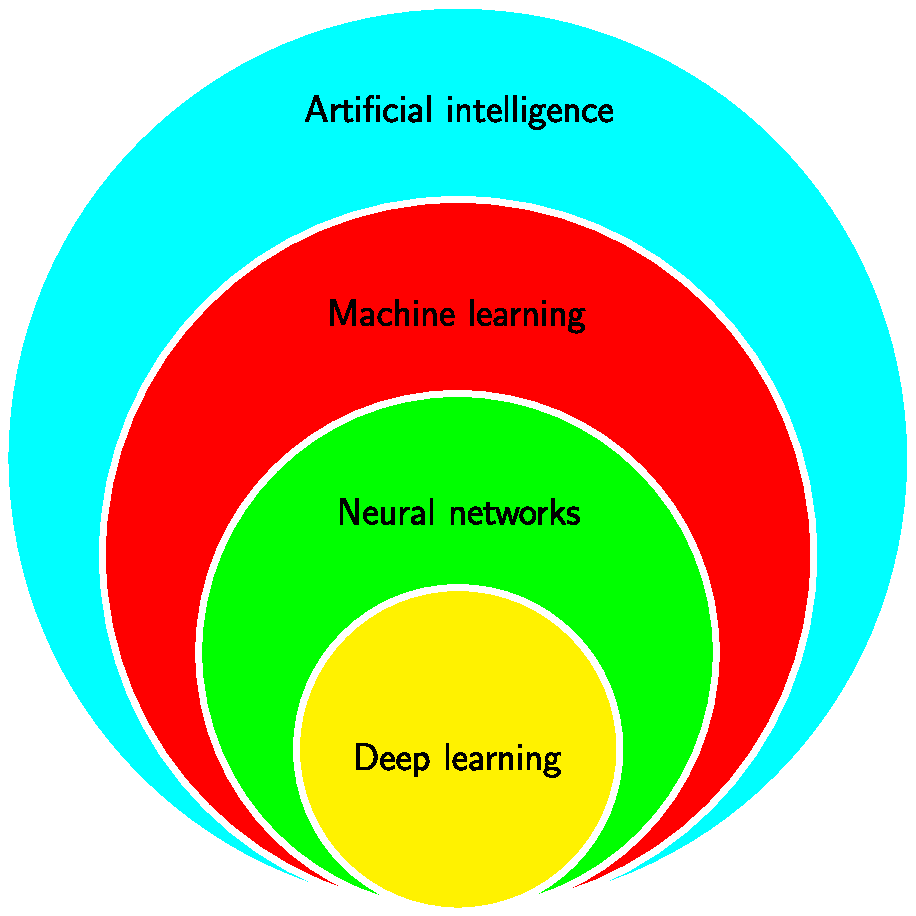
\includegraphics{chapterf00-01}
\end{marginfigure}

The newcomer can easily be confused by the terminology used in the field.  There is some differences in the details of different definitions, but the broad consensus can be depicted as fields of expertise within fields of expertise, often drawn as a Venn diagram as shown here.

\ac{AI} can be broadly defined as the simulation of human intelligence by machines, including computers. These \ac{AI} processes include learning, reasoning and self-correction. Work in this area started as early as the 1940s. \ac{ML}\cite{WikiPediaMachineLearning2019,DanielFaggella2019}, is normally defined as the application of \ac{AI} to learn from data without explicitly programming the learned behaviour. \ac{ML} therefore focuses on the development of programs that can access data and learn new behaviour from the data, by themselves.  Early ML work started in the 1980s. Arguably the neural networks subset does not belong to the figure, but this technology plays such a key role that perhaps it should earn to be explicitly shown.  Neural nets is a computing technique loosely modelled on the human brain, that can  recognise patterns.  These neural nets are a dominant part of the bigger machine learning field. Neural nets attracted much attention in the 1980's and 1990s, although it was used extensively, the application of this technology was limited by computing power.  In particular, the pattern information had to be carefully prepared for the neural net, which sometimes required very special skills. Practical application of neural nets were limited to three-layer neural nets, which could be trained by the then-available algorithms and computers.  \ac{DLea}\cite{WikiPediaDeepLearning2019}, which required more than three layer neural nets, with deeply hidden layers (hence the term deep learning) was defined and understood already in the 1980s.  The algorithms and computers could not solve the deep learning problems at the time.   Around 2006 new algorithms were was proposed that opened up the deep learning neural nets to practical use.
Deep learning is therefore a special application of neural nets, which is a part of machine learning, which in turn is part of artificial intelligence.

\newthought{Machine learning} is defined as\cite{DanielFaggella2019} ``Machine Learning is the science of getting computers to learn and act like humans do, and improve their learning over time in autonomous fashion, by feeding them data and information in the form of observations and real-world interactions.''


\section*{Historic Perspective}

In his excellent blog post \cite{Vazquez2018} Favio V\'{a}zquez gives a brief introduction to the history of \ac{DL} with a very nice historic time line (Figure~\ref{fig:deeplearningtimeline}).

\begin{figure*}[tph]
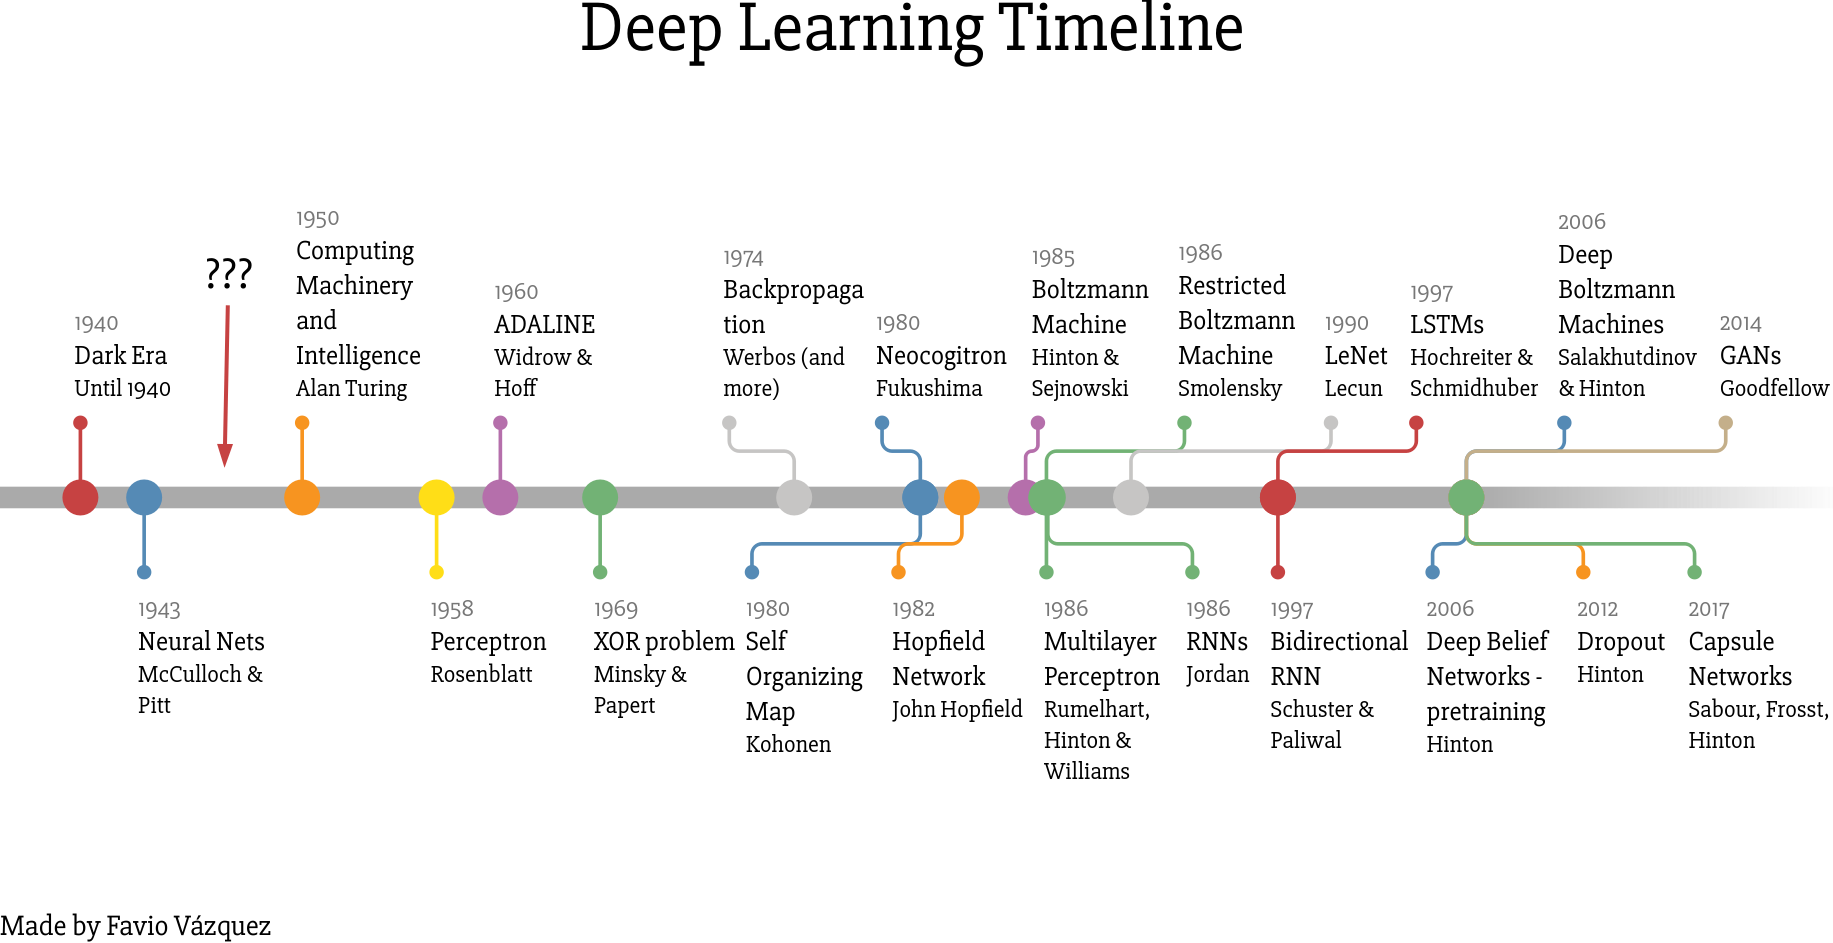
\includegraphics[width=\textwidth]{deeplearningtimeline}
\caption{Favio V\'{a}zquez's \ac{DL} time line}
\label{fig:deeplearningtimeline}
\end{figure*}



%\FloatBarrier

\section*{The Plan}

My present motivated plan to learn more about \ac{ML} is as shown below. This is the third plan since I started, which demonstrates the volatility of the \ac{ML} world. What seems like a good idea today is in insanely poor choice six months later.

\begin{enumerate}
\item \marginnote{A study \cite{Ericsson93therole} found that full mastery requires long and consistent practice, but another study \cite{Macnamara2014} found that practice alone is not a guarantee for success.} Select the technology/product with utmost care.  Provided you have the ability, it takes ten years or ten thousand hours to fully master a topic. How many ten-year cycles can you afford in your lifetime?

\item \marginnote{Even staying with large companies is risky. Google is notorious for dropping services. Do you remember the MFC technology from Microsoft? It is interesting that Qt, HTML, Python and JavaScript are still around after all these years.} You want to invest in a technology with a long shelf life (probably not possible in \ac{ML}). Stay with mainstream and large projects with a wide following. Stay away from small or risky projects, time spent there is time wasted. 
    
\item I want to stay on the Windows platform this is where all my tools are (I do not have a Linux boot PC at present).  This requirement severely limits my options (see below). Linux is miles ahead here, most of the serious work is done on Linux.
    
\item Stay local, not in the cloud.   If you have large models with large data sets, using the cloud services is far better, but I have no funding to pay for cloud services at this time.

\item Stay with open source projects with large following and a good Internet support base. The bigger the user base, the better you protect your investment in terms of support and long term survivability. Services such as StackOverflow provide more useful support than does commercial companies, simply because of the large support base. People often denigrate the value of YouTube, but there are also some seriously useful tutorials and support information there. 

\item Steps:
\begin{enumerate}
\item Start with Michael Nielsen's excellent introductory online book \cite{Nielsen2015}. His book is included as Part~I of this document.  The purpose with the book is to provide understanding at a conceptual level, not as a rigourous academic treatise; which is what I need to start of with. \marginnote{In the online version of the book, Nielsen provides interactive JavaScript tools which do not transfer well to a PDF document.  As an alternative, I coded some of the interactive functionality in Python notebooks, which are available on the GitHub page \cite{willersNNDLgithub2019}. I also sometimes add static screen shots from Nielsen's online tools.}
\item Start with Scikit Learn, simply because it is easily installable, does not require a \ac{GPU} software installation, has a large example base and is reasonably well documented.
\item Invest in learning TensorFlow \cite{TensorFlow2Alpha2019}.  I previously considered PyTorch \cite{paszkePyTorch2017,PyTorch2019} and fastai \cite{fastai2019}, but found it difficult to do a GPU install on Windows.  One of the objections against TensorFlow~1 was its awkward \lstinline{sessions}  construction, but this falls away with TensorFlow~2.  Google also integrated Keras \cite{cholletkeras2015,cholletkerasio2015} into TensorFlow~2 as a native higher-level framework.
    Installation of GPU TensorFlow~2 is still not simple for Windows, but I will start with the \ac{CPU} version. GPU functionality is readily available on Linux or on Google's online CoLaboratory \cite{GoogleCoLaboratory2019}.
\item Work through G\'{e}ron's book \cite{geron2017handson} \textit{Hands-on machine learning with Scikit-Learn and TensorFlow}.  The first part of the book uses Scikit Learn to establish a good understanding and then moves on to using the TensorFlow tools.
    The book receives good reviews and is presently under revision for a second edition, covering TensorFlow~2.
\item I want to document my learning process in Part~II of this book, and add insights from other authors into Part~III of this book. This will come as time availability allows.
\item For in-depth backup and if I ever need this, I will consult the academic books \cite{geron2017handson,Webb2002statpatn,Michie94,theodoridis2003,Duda2001,Bishop1995,Bishop2006,Goodfellow2016}, but for now, my interest is still at an elementary level.
\end{enumerate}
\item All of the above will be done at a leisurely pace outside of working hours and jointly with my life partner and fellow traveller Riana.
\end{enumerate}


\section*{Attribution}

\begin{enumerate}
\item 
The entirety of Part I is taken from Michael Nielsen's online book\cite{Nielsen2015}. Some minor changes were made to the text.

\item
The stylistic neuron on the Part header pages were adapted from \cite{Erler2004}. 

\item
Some of the neural diagrams  are created with the \lstinline{neural} TikZ module for \LaTeX{}\cite{cowan2019} by Mark Cowan.
\end{enumerate}
